\documentclass{article}
\usepackage[normalem]{ulem}
\usepackage[14pt]{extsizes}
\usepackage[utf8]{inputenc}
\usepackage[T2A]{fontenc}
\usepackage{amsmath}
\usepackage{amssymb}
\usepackage{mathtools}
\usepackage{hyperref}
\usepackage{amsfonts}
\usepackage{cmap}
\usepackage{multicol}
\usepackage{comment}
\usepackage[parfill]{parskip}
\usepackage{enumitem}

\usepackage{listings}
\usepackage{color}
\usepackage{colortbl}
\usepackage{xcolor}
\usepackage[left=1.5cm,right=2cm,top=2cm,bottom=2cm,bindingoffset=0.1cm]{geometry}
\usepackage[russian]{babel}
\usepackage[pdf]{graphviz}
\usepackage{tikz}
\usepackage{pgfplots}
\usepackage{dsfont}
\newcommand\dsone{\mathds{1}}

\usepackage{etoolbox}
\AtBeginEnvironment{enumerate}{\linespread{.84}\selectfont}
\newcommand{\ctd}{\begin{flushright} $\square$ \end{flushright}}

\usepackage{graphicx}
\setlength\fboxsep{3pt}
\setlength\fboxrule{1pt}
\pagenumbering{gobble}

\hypersetup{
    colorlinks=true,
    linkcolor=blue,
    filecolor=magenta,      
    urlcolor=blue,
    pdftitle={Alfo},
    pdfpagemode=FullScreen,
    }
\lstset{
  basicstyle=\footnotesize\ttfamily,
  numbers=left, 
  numberstyle=\footnotesize\color{black},
  stepnumber=0,
  numbersep=0.7em,
  backgroundcolor=\color{white!95!gray},
  showspaces=false,
  showstringspaces=false,
  showtabs=false,
  frame=single,
  rulecolor=\color{black},
  tabsize=4,
  %captionpos=b,
  breaklines=true,
  breakatwhitespace=false,
  %title=\lstname,
  identifierstyle=\color{black!50!green},  
  keywordstyle=\color{blue},
  commentstyle=\color{gray},
  stringstyle=\color{purple},
  escapeinside={\%*}{*)},
  morekeywords={n,k},
  morecomment=[l][\color{black!50!green}]{\#},
  morecomment=[s][\color{gray!50!black}]{/**}{*/}
}

\newcommand{\updownarrows}{\mathbin\uparrow\hspace{-.5em}\downarrow}
\newcommand{\downuparrows}{\mathbin\downarrow\hspace{-.5em}\uparrow}
\newcommand{\defeq}{\overset{\mathrm{def}}{=\joinrel=}}
\newcommand{\defLeftrightarrow}{\xLeftrightarrow{def}}

\title{Дискретная математика, 1 курс}
\author{Амосов Алексей, Давыдов Иван, М3138}
\date{2024-2025}

\begin{document}
\maketitle
\tableofcontents
\pagebreak

\section{Лекция 1}
\subsection{Введение определний}
Множество - неопределенное понятие. A - какое-то множество. Мы умеем понимать:

$x \in A$ или $x \notin A$ 

В множестве несколько одинаковых элементов быть не может(вопрос бессмысленен:  $\forall x, \forall A: x \in  A  $ или $ x \notin A).$

Будем считать, что есть $U$ ("универсум") и все множества в нем лежат.

Мы можем спокойно работать с множеством натуральных, целых, рациональных, вещественных, иногда комплексных. Обычно будет понятно из контекста какой у нас универсум.

$\mathbb{B}$ = \{0,1\}

$C:=\{x \in A: P(x) = 1\}$, где P(x) - булевая функция.

C множеством можно делать много операций:

\textbf{1) Объединение}

$A \cup B = \{x: x \in A$  или $x \in B \}$

\textbf{2) Пересечние}

$A \cap B = \{x: x \in A$ и $x \in B \}$

\textbf{3) Вычитание}

$A \textbackslash B = \{x: x \in A$ и $x \notin B \}$

\textbf{4) Исключающее объединение (xor)}

$A \oplus B = (A \textbackslash B) \cup (B \textbackslash A)$

\textbf{5) Отрицание}

$\bar{A} = U \textbackslash A$

\textbf{Произведение множеств:}

Декартово произведение X и Y обозначается $X \times Y$, на языке кванторов:

 $X \times Y = \{(x,y):x \in X, y \in Y\}$ 
 
$A \times A = A^2$

$(A \times B) \times C = A \times (B \times C)$ --- пренебрегаем проблемой несоответсвия типов:
Вместо $\{a, \{b, c\}\}$ и $\{\{a, b\}, c\}$ считаем их равными $\{a, b, c\}$
На языке С++ вместо $pair(a, pair(b, c))$  и $pair(pair(a, b), c)$  воспринимаем элементы объединения как $tuple(a, b, c)$

\textbf{Функция} 

$f:A \rightarrow B$

$X \subset Y$ --- "мн-во X содержится в Y"; равносильно $x \in X: x \in Y$

$f \subset A \times B$. Выполнено $\forall x\, \exists!\,y \in B: (x,y) \in f$

$B^A = \{f:A \rightarrow B\}$ - множество, переводящие A через функцию

$2^{A}=\mathbb{B}^{A}$ -каждому элементу сопоставили 1 или 0. Удобно брать подмножества

\textbf{Инъекция.} Если $x \neq y$, то $f(x) \neq f(y)$

\textbf{Сюръекция.} $\forall y \in B: \exists x: f(x)=y$

\textbf{Биекция} = Инъекция + Сюръекция = Взаимнооднозначное соотвествие

$\varnothing$ - пустое множество

$A^0 = \{<>\}$ - пустой картеж = void = множество с ничего внутри

$\varnothing \times A = \varnothing$

$1 \times A = A$ - зачем-то приклеили  каждому элементу ничего

\subsection*{Отношения}

(бинарные) отношения между A и B

$R \subset A \times B$

$A,B = \mathds{N}$

$< = \{(a,b): a<b\}$ Обозначается aRb.

$<$ - такое отношение, что A должно быть меньше B.

$R \subset A \times A$ - отношение на A.

Отношения можно отображать в виде ориентированных графов.
Виды отношений: 

1) \textbf{Рефлексивность}.

$\forall x \in A: aRa$, то есть (a,a) входит в наше отношение.

2) \textbf{Антирефлексивность}.

$\forall x \in A: a\textbackslash Ra$, то есть (a,a) не входит в наше отношение.

3) \textbf{Симметричность}.

Если $aRb$, то $bRa$.

4) \textbf{Антисимметричность} 

Если $a\neq b$ и $aRb$, то $a\textbackslash Rb$.

5) \textbf{Транзитивность}.

Если $aRb$ и $bRc$, то $aRc$.

\textbf{Классы отношений.}

Отношения частичного порядка - 1,4,5 (строгий 2,4,5).

Отношения линейнего порядка - частичный и $\forall a,b: aRb$ или $bRa$.

Отношения полного порядка - линейный и $\forall $множество X имеет min элемент.

Отношения эвивалентности - 1,3,5.

$X,R$ - эквивалентна на $X$, тогда $A\in X /R$

\section{Лекция 2}
\subsection{Композиция}
Пусть есть бинарные отношения $ R \subset X \times Y $; $ S \subset Y \times Z $.
Композиция $T = RS$. 
\textbf{Определение композиции:} 
$ xTy \defLeftrightarrow \exists z : xRz, zSy$.
"Есть такой z, что через него можно добраться из x в y (Следовательно, композиция \textit{не коммутативна}, $ RS \neq SR $)"
\textbf{С точки зрения графов:}
"Есть такая вершина, z, что можно по ней пройти сначала по ребру, соответствующему отношению R, потом по ребру, соответствующему ребру S"
\textbf{Пример:} 
Пусть $ R \subset X\times Y$ - отношение "человек x владеет собакой y", а $ S \subset Y\times Z$ - отношение "собака y носит ошейник x", тогда композиция $T=RS$ будет отношением "собака человека x носит ошейник z"
\begin{center}
  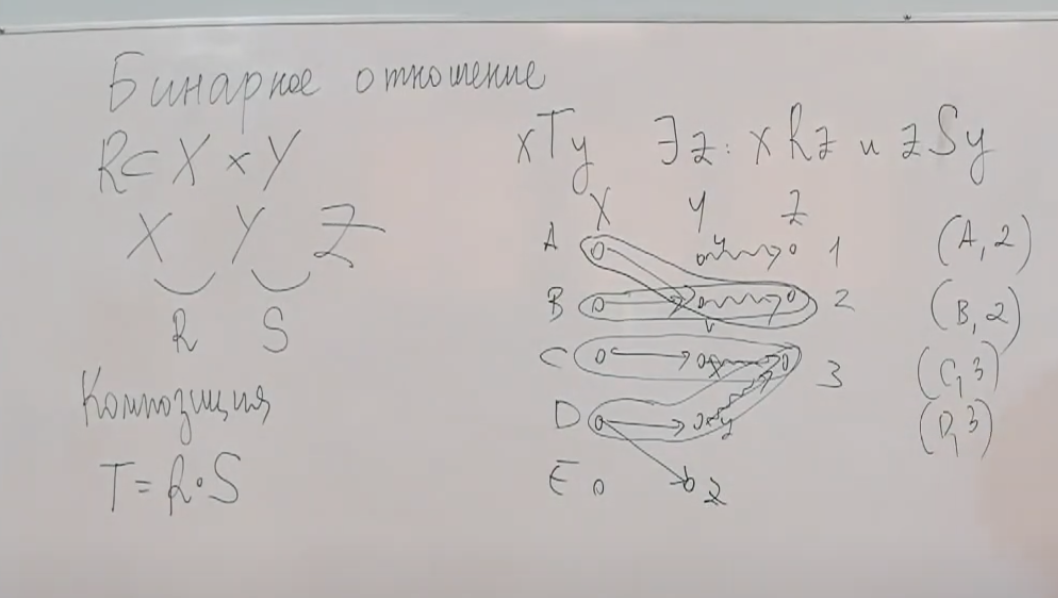
\includegraphics[height=8cm]{2-1-1.png}
\end{center}
Следовательно, присутствует \textit{ассоциативность}: $ T = (AB)C = A(BC) $

Композиция с собой: два элемента (вершины) находятся в отношении-композиции $ R^{n} $, если между ними имеется путь длины ровно n.

\subsection{Транзитивное замыкание} 
Пусть R - отношение "быть родителем", тогда отношение "быть предком" - транзитивное замыкание R (обозначается $ R^{+} $)
\[R^{+} = \overset{\inf}{\underset{k=1}{U}}R^{k}\]
Если вершина должна включать себя в замыкание (например R - "быть сыном в дереве", а $R^{*}$ - "иметь на поддереве"), то следует объединить с $R^{0}$
\[R^{0} = (x, x): x \in X; \]
Это называется \textit{рефлексивно-транзитивным замыканием} и обозначается $R^{*}$
\[R^{*} = \overset{\inf}{\underset{k=0}{U}}R^{k}\]

$R^{+}$ и $R^{*}$ транзитивны:
$ \newline
xR^{*}y \rightarrow xR^{i}y \newline 
yR^{*}z \rightarrow yR^{j}z \newline
$Следовательно, $ xR^{i+j}z \newline 
$ А т.к. объединяем до бесконечности, $(i+j) \in [0; \inf) $, Значит из $ xR^{*}y; yR^{*}z $ следует $ xR^{*}z $, что является определением транзитивности.
Более того, из всех транзитивных отношений S, для которых верно $ R \subset S $, $R^{+}$ является минимальным (с наим. количеством ребер).
Иначе говоря, $\forall T$, где T транзитивно и $R \subset T$, $R \subset T$, выполнено $R^{+} \subset T$ \newline
Док-во по индукции:\newline
База: $R \subset T$, т.к. это дано.\newline
Докажем, что из $ R^{i} \subset T $ следует $ R^{i+1} \subset T $ \newline
$ xR^{i+1}y \leftrightarrow x(R^{i}R)y \rightarrow \exists z: xRz, zR^iy $ по определению \newline
$ \rightarrow xTz, zTy$, а т.к. отношение T транзитивно, $xTy$ \newline То есть $ R^{i+1} \subset T $, ЧТД

\subsection{Булевые функции:}
$ \mathbb{B} $ - множество из двух элементов ({0, 1} или {false, true}, {орёл и решка} и т.д.)

Функция f, принимающая n элементов, принимает декартово произведение множеств, из которых берутся элементы:
\[ f: A_1 \times A_2 \times ... \times A_n \longrightarrow B\]

Определение булевой функции:
\[ f: \mathbb{B}^{n} \longrightarrow \mathbb{B}\]
Позже \( f: \mathbb{B}^{n} \longrightarrow \mathbb{B}^{k}\)
(В данном случае можно рассматривать как k отдельных булевых функций $f_1, f_2, ..., f_k$)

\subsubsection{n = 0}
$ \mathbb{B}^{0} = \{[]\}, $ то есть мощность 1.
Функций, принимающих void и возвращающих boolean две: $\mathbf{0}$ и $\mathbf{1}$ ("тождественный 0 и 1 соответственно") % 1 и 0 должны быть с черточкой как у множеств натуральных числ, рациональных, действительных и т.п.

\subsubsection{n = 1}
Функций, принимающих boolean и возвращающих boolean четыре: \newline
$0 \rightarrow 0 \newline$
$0 \rightarrow 1 \newline$
$1 \rightarrow 0 \newline$
$1 \rightarrow 1 \newline$

Свойство функции принимать k аргументов - "арность" (arity)
(Унарность, бинарность, тернарность...)

$f(0) = 0 \newline$
$f(1) = 1$ - тождественная функция (identity function)

$f(0) = 1 \newline$
$f(1) = 0$ - функция отрицания (не x, not x, !x...)

\subsubsection{n = 2}
Всего 16 возможных функций (бинарные ф-ии - одни из основных)
Общая формула количества возможных функций: $ 2^{2^{n}}$

\begin{table}
    \centering
    \begin{tabular}{ |c|c|c|c|c|c|c|c|c|c| }
        \hline
         x & y & $\mathbf{0}$ & AND & $!(x \impliedby y)$ & x & y & !$(x \implies y)$ & XOR & OR \\
         \hline
         0 & 0 & 0 & 0 & 0 & 0 & 0 & 0 & 0 & 0 \\
         0 & 1 & 0 & 0 & 0 & 0 & 1 & 1 & 1 & 1 \\
         1 & 0 & 0 & 0 & 1 & 1 & 0 & 0 & 1 & 1 \\
         1 & 1 & 0 & 1 & 0 & 1 & 0 & 1 & 0 & 1 \\
         \hline
    \end{tabular}
    \label{tab:my_label}
\end{table}

\begin{table}
    \centering
    \begin{tabular}{ |c|c|c|c|c|c|c|c|c|c| }
        \hline
         x & y & NOR & $x = y$ & $!y$ & $x \impliedby y$ & !x & $x \implies y$ & NAND & $\mathbf{1}$ \\
         \hline
         0 & 0 & 1 & 1 & 1 & 1 & 1 & 1 & 1 & 1 \\
         0 & 1 & 0 & 0 & 0 & 0 & 1 & 1 & 1 & 1 \\
         1 & 0 & 0 & 0 & 1 & 1 & 0 & 0 & 1 & 1 \\
         1 & 1 & 0 & 1 & 0 & 1 & 0 & 1 & 0 & 1 \\
         \hline
    \end{tabular}
    \caption{Все бинарные функции}
    \label{tab:my_label}
\end{table}

Таблица в исполнении Станкевича:
\begin{center}
  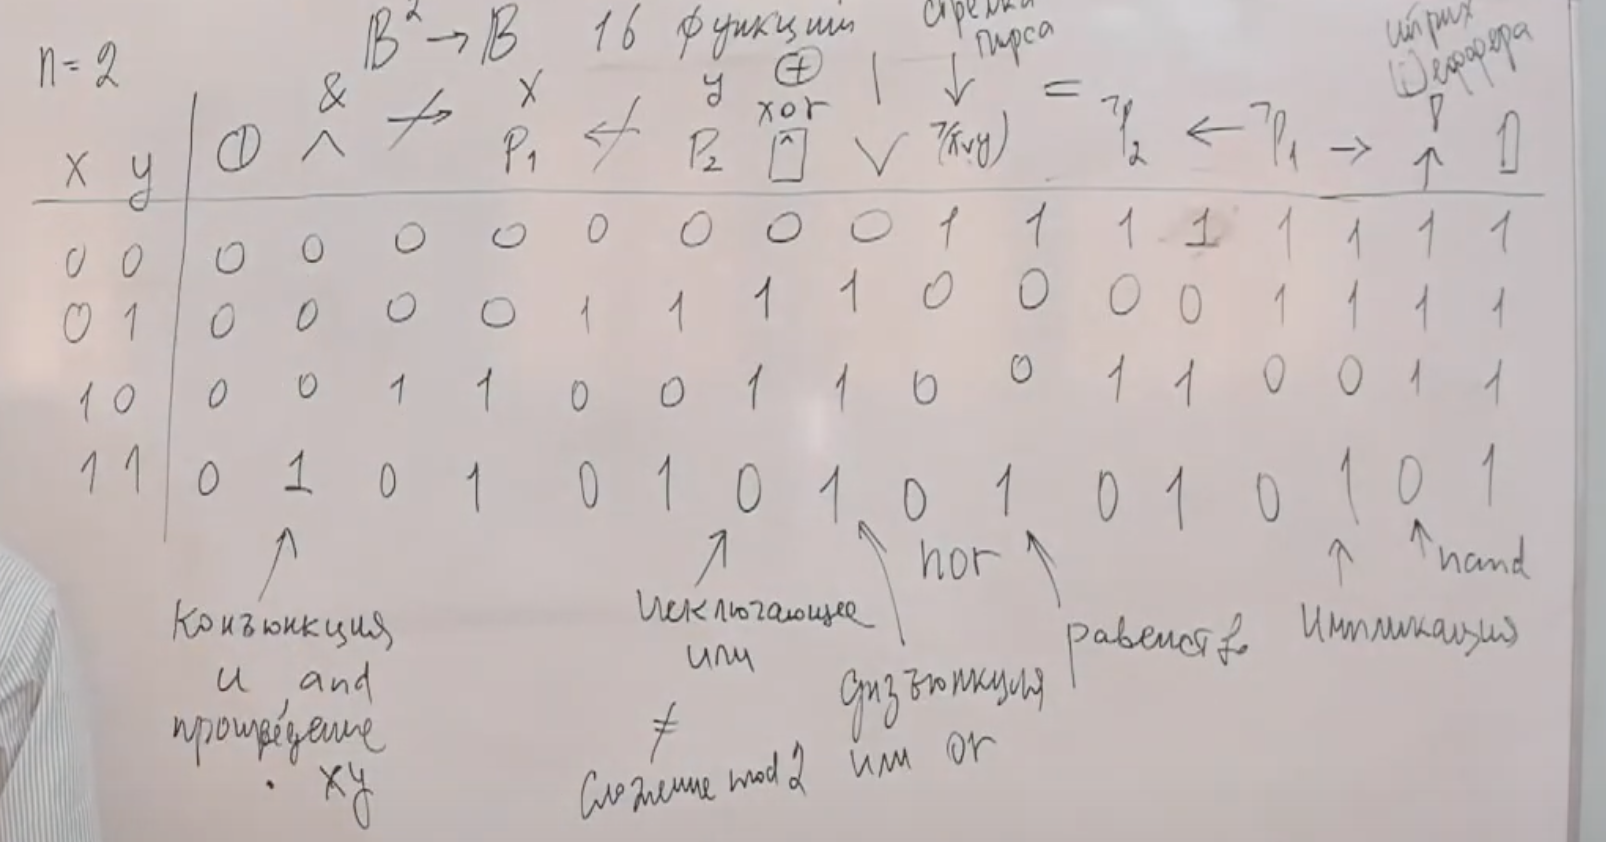
\includegraphics[height=9.1cm]{2-2-1.png}
\end{center}

\subsubsection{n = 3}
tldw.
Из интересных - медиана, она же "голосование" (возвращает тот аргумент, которого больше, см. таблица 2)


\begin{table}
    \centering
    \begin{tabular}{ |c|c|c|c| }
        \hline
         x & y & z & med \\
        \hline
         0 & 0 & 0 & 0 \\
         0 & 0 & 1 & 0 \\
         0 & 1 & 0 & 0 \\
         0 & 1 & 1 & 1 \\
         1 & 0 & 0 & 0 \\
         1 & 0 & 1 & 1 \\
         1 & 1 & 0 & 1 \\
         1 & 1 & 1 & 1 \\
        \hline
    \end{tabular}
    \caption{Таблица истинности медианы}
\end{table}

\subsubsection{Задание булевых функций}
1) Таблица истинности (плюс: есть у всех функций, прямолинейный способ; минус: асимптотика по памяти $(2^{2^{n}})$ \newline
2) Задание формулой (некой строкой): пусть мы выбрали некоторые базисные функции (системя связок), например AND, OR, NOT, XOR. Для каждой базисной функции возьмем обозначение.

Каноническое обозначение: 
f(x, y)

Инфиксное обозначение:
x f y (необходимо задавать приоритеты выполнения функций)

Пример: импликация - OR(NOT(x), y)

\textbf{"Замыкание множества функций F"} - множество всех функций, которые можно составить, используя функции из множества F (обозначается как $\overline{F}$)

Например, $\textbf{0} \in \overline{XOR}$, но $\textbf{1} \notin \overline{XOR}$

\textbf{Теорема о стандартном базисе:} 
\[ \overline{\{AND, OR, NOT\}} = \mathbb{BF} \] ($\mathbb{BF}$ --- множество всех булевых функций). Более того, можно избавиться от AND или OR (см. закон де Моргана). Доказательство - существование СКНФ/СДНФ для любой таблицы истинности (тождественный 0 не имеет СДНФ, но можно выразить просто как NOT(OR(A,A)) или AND(A, NOT(A))). 


(Пасхалко: есть по крайней мере одна базисная функция F из таблицы 1, для которой справедливо $ \overline{F} = \mathbb{BF} $. Можете догадаться, какая? Почему? Есть ли другие?) 

\subsection{Конъюктивная нормальная форма}
\href{https://ru.wikipedia.org/wiki/%D0%9A%D0%BE%D0%BD%D1%8A%D1%8E%D0%BD%D0%BA%D1%82%D0%B8%D0%B2%D0%BD%D0%B0%D1%8F_%D0%BD%D0%BE%D1%80%D0%BC%D0%B0%D0%BB%D1%8C%D0%BD%D0%B0%D1%8F_%D1%84%D0%BE%D1%80%D0%BC%D0%B0}{Конъюктивная нормальная форма}

\subsection{Дизъюнктивная нормальная форма}
\href{https://ru.wikipedia.org/wiki/%D0%94%D0%B8%D0%B7%D1%8A%D1%8E%D0%BD%D0%BA%D1%82%D0%B8%D0%B2%D0%BD%D0%B0%D1%8F_%D0%BD%D0%BE%D1%80%D0%BC%D0%B0%D0%BB%D1%8C%D0%BD%D0%B0%D1%8F_%D1%84%D0%BE%D1%80%D0%BC%D0%B0}{Дизъюнктивная нормальная форма}
\section{Лекция 3}
\subsection{Базисы}

\textbf{Базис} - набор булевых функций.

\textit{F} называется \textbf{полным базисом}, если используя только булевые функций из \textit{F} мы можем задать любую булеву функцию. Пример:

$\{\wedge, \vee, \neg\}$ ---  стандартный полный базис. Можем выкинуть $\wedge$ либо $\vee$ 
 и он останется полным базисом.

\textbf{Теорема.} Пусть $F$ - полный базис. $G$ - множество функций.
$\forall f \in F:$ можно задать формулой над $G$.
Тогда G - полный базис.

\begin{enumerate}

\item[] \uline{Доказательство.}

Так как $F$ - базис, через него можно выразить любую булеву функцию. Тогда давайте рассмотрим дерево операций над $F$ для какой-то булевой функции и докажем, что для этой булевой функции мы можем построить дерево операций над $G$. Возьмем дерево операций над $F$ и рассмотрим его конкретную вершину. Это какая-то функция $f$, про которую мы знаем, что $f \in F$. Раз так, то мы можем заменить ее на ее формулу над $G$. Сделаем так со всеми вершинами в дереве операций над $F$ и получим дерево операций над $G$. Раз над $G$ можно задать любую функцию, то $G$ - базис. Q.E.D.

\end{enumerate}

Так мы можем доказать, что $\{\vee, \neg\}$, $\{\wedge, \neg\}$ - полные базисы.

\subsection{Полином Жегалкина}

$\{\wedge, \oplus, 0\}$ --- \textbf{арифметический базис.}

Выражение булевой функции в арифметическом базисе --- \textbf{полином Жегалкина}.

Приведенный полином Жегалкина --- вид полинома Жегалкина, в котором опущены все произведения с 0. 

\textbf{Теорема.}  $\forall$ функции $\exists!$ приведенный полином Жегалкина
\begin{enumerate}
\item[] \uline{Доказательство.}
Всего функций от n переменных - $2^{n^n}$. Полиномов Жегалкина  $2^{n^n}$. Каждой функции соответсвует полином Жегалкина. У нас не может быть двух записей в виде полинома Жегалкина для одной и той же функции. Доказывается это от противного, если у нас есть два разных полинома Жегалкина  $Q_1$ и $Q_2$, которые задают одну и ту же функцию, то $Q_1\oplus Q_2 = 0$. Но раз $Q_1$ и $Q_2$ не совпадают, то $Q_1\oplus Q_2\neq0$. Тогда это биекция между двумя множествами. Q.E.D.
\end{enumerate}



\subsection{Классы Поста}
Классы Поста - это свойства булевых функций, такие, что если мы работаем над базисом, все функции которого принадлежат какому-то классу Поста, то и все функции, достижимые из этого базиса, также лежат в этом классе Поста.

\textbf{Классы Поста}:
\begin{enumerate}
    \item[1.] \textbf{Сохраняющие 0} - булевы функции, которые от входного набора состоящего только из 0 выдают 0.  $\{\vee, \wedge\}$ --- сохраняют ноль.
    
    Очевидно, любая функция над базисом из функций, сохраняющий 0 также будет сохранять 0.
    \item[2.] \textbf{Сохраняющие 1} - булевы функции, которые от входного набора состоящего только из 1 выдают 1.  $\{\vee, \wedge\}$ --- сохраняют один. 
    
    Также очевидно, что любая функция над базисом из функций, сохраняющий 1 также будет сохранять 1.
    \item[3.] \textbf{Линейность} - функция линейна, если ее представление в виде полинома Жегалкина не имеет в записи $\wedge$. 
    
    Доказательство линейности функции над базисом, состоящим из линейных функций также очевидно, если представить данную функцию в виде полинома Жегалкина, это упражнение я оставлю читателю.
    \item[4.] \textbf{Монотонность} - функция монотонна, если при увеличении любого аргумента результат не уменьшается, то есть $\forall$ 2 наборов аргументов $x_1, \ldots, x_n$ и $y_1, \ldots, y_n$, таких, что $x_i\leq y_i$, верно $f(x_1,x_2, \ldots, x_n) \leq f(y_1,y_2, \ldots, y_n)$ .
    
    Доказательство монотонности функции над базисом, состоящим из монотонных функций: Рассмотрим дерево операций для функии $f$, которая построена над базисом из монотонных функций. Тогда рассмотрим увеличение какого-то аргумента и докажем, что в этом случае значение $f$ не уменьшится. Предположим это не так, значит значение в корне уменьшилось. Но так как в корне у нас монотонная функция, то значение какого-то из его сыновей уменьшилось. Продолжим этот спуск и получим, что значение какого-то аргумента уменьшилось. Противоречие. Q.E.D. 
    \item[5.] \textbf{Самодвойственность} - функция самодвойственна, если $\forall$ набора аргументов $x_1, \ldots x_n$, верно  $F(x_1, \dots x_n)\neq F(\overline{x_1} \dots \overline{x_n})$. самодвойственности функции над базисом, состоящим из самодвойственных функций. Рассмотрим дерево операций для функии $f$, которая построена над базисом из самодвойственных функций. Тогда рассмотрим изменение всех аргументов и докажем, что в этом случае значение $f$ также изменится. Начнем рассматривать вершины снизу вверх. Так как каждая вершина - это самодвойственная функция, и все аргументы поменялись на противополжные, то значение и в этой вершине сменится. Тогда по итогу в корне значение также сменится на противоположное. Q.E.D. 
\end{enumerate}
\subsection{Критерий Поста}
$F$ --  полный базис $\Leftrightarrow$ нем есть не самодвойственная, не сохраняющая ноль, не сохраняющая один, не линейная, не монотонная.

\begin{enumerate}
\item[] \uline{Доказательство.}
\item[1)] Заметим, что необходимость этого утверждения была доказаны выше для каждого класса отдельно.

 \item[2)]Докажем, что если набор F не содержится полностью ни в одном из данных классов, то он является полным.

\begin{enumerate}
    \item  Рассмотрим функцию, не сохраняющую ноль --- $f_0$. Тогда $f_0(1)$ может принимать два значения:
     \begin{enumerate}
        \item[1.] $f_0(1)=1$, тогда $f_0(x,x,x,\ldots,x)=1$
        \item[2.] $f_0(1)=0$, тогда $f_0(x,x,x,\ldots,x)=\neg x$

.
    \end{enumerate}
    \item Рассмотрим функцию, не сохраняющую один — $f_1$. Тогда $f_1(0)$ может принимать два значения:
    \begin{enumerate}
        \item[1.]$f_1(0)=0$, тогда $f_1(x,x,x,\ldots,x)=0$
        \item[2.]$f_1(0)=1$, тогда $f_1(x,x,x,\ldots,x)=\neg x$
    \end{enumerate}
    Таким образом, возможны четыре варианта:
    \begin{enumerate}
        \item[a2b2.] Мы получили функцию $\neg$.
        Используем несамодвойственную функцию $f_s$. По определению, найдется такой вектор $x_0$, что $f_s(x_0)=f_s(\overline{x_0})$. Пусть $x_0=(x_{0_1},x_{0_2},\ldots,x_{0_k})$.
        
        Рассмотрим $f_s(x^{x_{0_1}},x^{x_{0_2}},\ldots,x^{x_{0_{k}}})$, где либо $x^{x_{0_i}}=x$, при $x_{0_i}=1$. Либо $x^{x_{0_i}}=\neg x$, при $x_{0_i}=0$. Нетрудно заметить, что $f_s(0)=f_s(1) \Rightarrow  f_s=const$. Таким образом мы получили одну из констант. Можем получить вторую, взяв отрицание от первой.

        \item[a2b1.] Мы получили $\neg$ и 0$\Rightarrow$ имеем константу, равную 1, поскольку $\neg 0=1$

        \item[a1b2.] Мы получили $\neg$ и 1$\Rightarrow$ имеем константу, равную 0, поскольку $\neg 1=0$

        \item[a1b1.] Мы получили 1 и 0. Рассмотрим немонотонную функцию $f_m$. Существуют такие $x_1,x_2,\ldots,x_n$, что $f_m(x_1,x_2,\ldots,x_{i-1},0,x_{i+1},\ldots,x_n)=1$, 
        $f_m(x_1,x_2,…,x_{i-1},1,x_{i+1},\ldots,x_n)=0$, зафиксируем все $x_1,x_2,…,x_n$, тогда $fm(x_1,x_2,…,x_{i-1},x,x_{i+1},\ldots,x_n)=\neg x$.  Такие   $x_1,x_2,\ldots,x_n$ являются x-ами при которых ломается монотонность

    \end{enumerate}
    В итоге  имеем три функции: $\neg, 0, 1$ в каждом из случаев. Покажем, что из них можно получить или или и.

    Используем нелинейную функцию $f_l$. Среди нелинейных членов $f_l$
 (ее представления в виде полинома Жегалкина), выберем тот, в котором минимальное количество элементов. 
 
 Все аргументы кроме двух в этом члене приравняем единице, оставшиеся два назовем $x_1$
 и $x_2$. 
 
 Все элементы, не входящие в данный член, примем равными нулю. Тогда эта функция будет представима в виде $g_l=x1x2[\oplus x1][\oplus x2][\oplus 1]$ 
, где в квадратных скобках указаны члены, которые могут и не присутствовать (остальные слагаемые будут равны нулю, поскольку в них есть как минимум один аргумент, не входящий в выбранный член, так как в выбранном члене минимальное число элементов).

Рассмотрим несколько вариантов:

\begin{enumerate}
    \item[1)] Присутствует член  $\oplus 1$.
    
    Возьмем отрицание от $g_l$ и член $\oplus 1$ исчезнет.
    \item[2)] Присутствуют три члена, без $\oplus 1:$
    
    $ g_l=x1x2\oplus x1 \oplus  x2$. Составив таблицу истинности для этой функции нетрудно заметить, что она эквивалентна функции или.
    \item[3)] Присутствуют два члена, без  $\oplus 1$.
    
    Построив две таблицы истинности для двух различных вариантов, заметим, что в обоих случаях функция истинна только в одной точке, следовательно, СДНФ функции $g_l$
 будет состоять только из одного члена. Если это так, то не составляет труда выразить или через не
 и $g_l$.
    \item[4)] Присутствует один член.
     Выразим $\wedge$ через $\neg$ и $g_l$ аналогично пункту 3.
\end{enumerate}

В итоге получим функцию $\neg$ ,а также функцию или либо и. Любую булеву функцию, не равную тождественному нулю, можно представить в форме СДНФ, то есть выразить в данном базисе.

Значит, полученные функции образуют полную систему, поскольку с их помощью можно выразить любую булеву функцию. Из этого следует, что F — полная система функций, что и требовалось доказать.

\end{enumerate}
\end{enumerate}

\section{Лекция 4}

\subsection{Преобразование Мёбиуса}
Преобразование Мёбиуса позволяет переводить коэффиценты из полинома Жегалкина в таблицу истинности и наоборот. 

\begin{center}
  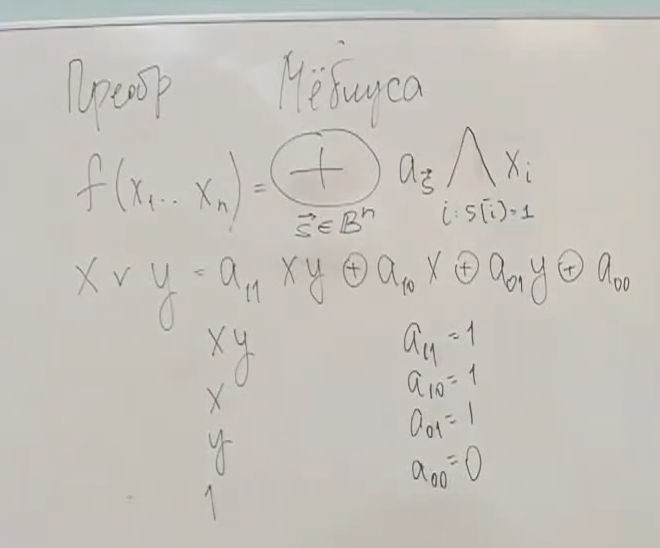
\includegraphics[height=9.1cm]{Mebius.png}
\end{center}
  

Давайте заведем бинарные коэффиценты для полинома Жегалкина, которые будут отражать, берем мы или не берем то или иное слагаемое. Всего таких коэффицентов будет $2^n$, столько же, сколько и всего возможных членов полинома Жегалкина. Пронумеруем их так, если в члене нашего полинома есть $i$ый член, то в индексе коэффицента на $i$ом месте будет 1, иначе 0 (например для произведения $xz$ в полинома Жегалкина для функции от трех переменных индекс коэффицента будет 101). Получаем, что индекс коэффицента - булевый вектор какой-то длины, а его уже можно однозначто перевести в числовой коэффицент через двоичную систему счисления.
\newpage
Посмотрим на формулу с картиночки и начнем осознавать, откуда она взялась:
$\displaystyle f(x_1\dots x_n) = \bigoplus\limits_{\overrightarrow{s}\in\mathbb{B}^n}a_{\overrightarrow{s}}\bigwedge\limits_{i:s[i]=1}x_i$ - это просто формула полинома Жегалкина. Давайте разберемся, когда у нас $a_{\overrightarrow{s}}\bigwedge\limits_{i:s[i]=1}x_i=1$, очевидно это происходит, только в том, случае, если выполняется это: $\forall i : s[i] = 1, x_i = 1$. Назовем такое отношение \textbf{доминированием} и будем обозначать как $\leq$.
Тогда нашу формулу можно переписать как: $$\bigoplus\limits_{\overrightarrow{s}\in\mathbb{B}^n}a_{\overrightarrow{s}}\bigwedge\limits_{i:s[i]=1}x_i = \bigoplus\limits_{\overrightarrow{s}\leq \overrightarrow{x}} a_{\overrightarrow{s}}$$ 

Отлично у нас получилась формула перехода от одного базиса к другому, и, как и в линейной алгебре, ее можно записать с помощью матрицы перехода, независимо от того, какие функции у нас были. Например для четырех переменных она выглядит так:

\parbox{\textwidth}{
    \centering
    \begin{tabular}{ |c|c|c|c| }
        \hline
         1 & 0 & 0 & 0 \\
        \hline
         1 & 1 & 0 & 0 \\
        \hline
         1 & 0 & 1 & 0 \\
        \hline
         1 & 1 & 1 & 1 \\
        \hline
    \end{tabular}
}


При умножении данной таблицы на коэффиценты в полиноме Жегалкина, мы получим таблицу истинности, сейчас мы докажем, что при повторном умножении, мы обратно получим коэффиценты полинома Жегалкина, то есть докажем, что такая таблица обратна сама себе.

Давайте доказывать, хотим такую формулу: $$a_t=\bigoplus\limits_{x\leq t}f_x $$ Но мы уже знаем, что верно: $$\bigoplus\limits_{x\leq t}f_x = \bigoplus\limits_{x\leq t}\bigoplus\limits_{s\leq x}a_s=\bigoplus\limits_{x,s : s\leq x \leq t}a_s$$
Хорошо тогда давайте разберемся сколько раз мы взяли конкретный $s$. Если $t$ не доминирует над $s$, то очевидно 0. Иначе мы взяли $a_s$ 2 в степени количества битов $i$, таких что в $t[i]=1$ и $s[i]=0$. Очевидно что это число нечетное, только если их 0, то есть на самом деле $a_s$ влияет на сумму, только если $s=t$, а значит справа у нас изначально было написано $a_t$. \textit{QED}.

\subsection{Функциональные элементы}
Рассмотрим новый способ представления булевых схем - в виде ориентированного графа. Вершины в нем - это булевые значения, а ребра - операции с ними. 

$Глубина схемы$ - длина максимального пути между вершиной, названной входной и вершиной, названной выходной. 

\subsubsection{Топологическая сортировка}
\textbf{Топологическая сортировка} - такая сортировка вершин ориентированного графа, что если в ней вершина $u$ стоит раньше вершины $v$, то не сушествует ребра из $v$ в $u$.

\textbf{Теорема.} Топологическая сортировка существует, если в графе нет циклов и наоборот.

В левую сторону доказать совсем легко, если в графе есть цикл и топологическая сортировка в нем тоже существует, то мы можем найти самую правую вершину этого цикла в топологической сортировке и тогда ребро из нее будет вести влево, что противоречит определению топологической сортировки.

В правую сторону доказать немного сложнее, но все также нетрудно. Найдем вершину, из которой не ведет ни одного ребра в другие вершины, если такой нет, то цикл обязательно существует ведь мы можем запуститься из любой вершины и ходить по ребрам, пока не вернемся в уже посещенную вершину и получим цикл. Тогда удалим эту вершину, а в топологическую сортировку допишем ее слева, что не может сломать ее, ведь из этой вершины нет ни одного ребра в те, которые мы допишем позже. Продолжая этот алгоритм, мы и получим топологическую сортировку. 

\section{Лекция 5}
\subsection{Сумматор}
Я пропущу сборку обычного сумматора, для него вам нужно просто придумать 2 схемы - битовый сумматор без переполнения и с переполнением и использовать второй $n$ раз.

\subsection{Двоичный каскадный сумматор}
Примечателен этот вариант сумматора тем, что имеет глубину $O(\log_2n)$. 

Чтобы его собрать для начала разберемся с тем, как устроен битовый сумматор с переполнением. 
\begin{enumerate}
    \item Если в нем складываются биты 0 и 0, то неважно, что ему пришло в качестве переполнения, он передаст далее 0, этот вариант мы назовем k.
    \item Если в нем складываются биты 1 и 0, то он передаст дальше то, что пришло ему в качестве переполнения, этот вариант мы назовем p.
    \item Если в нем складываются биты 1 и 1, то неважно, что пришло ему в качестве переполнения дальше он передаст 1, этот вариант мы называем g. 
\end{enumerate}

Тогда мы можем завести операцию композиции на этих вариантах, таблица которой будет выглядеть так:
\begin{center}
    \begin{tabular}{ |c|c|c|c| }
        \hline
         1\textbackslash2 & k & p & g \\
        \hline
         k & k & k & g \\
        \hline
         p & k & p & g \\
        \hline
         g & k & g & g \\
        \hline
    \end{tabular}
\end{center}

Тогда, если мы сможем быстро считать переполнение, которое приходит к конкретному биту, то и чему равен бит в итоге, узнать будет несложно. Чтобы насчитывать такое и получить логарифмическую глубину мы возьмем за основу структуру дерева отрезков, только теперь она будет работать немного по-другому. 
\begin{center}
  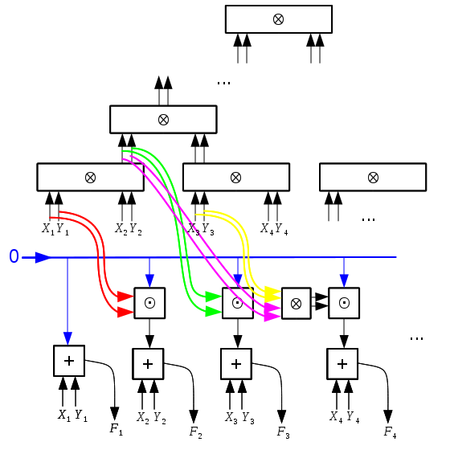
\includegraphics[height=9.1cm]{summ.png}
\end{center}
Функции у конретной вершины в дереве будут такие:
\begin{enumerate}
    \item Получить от предка копозицию прошлых переполнений, которые не являются частью этого поддерева(если корень то получить k).
    \item Если вершина является листом, то передать полученную от предка композицию дальше в алгоритм, а предку вернуть значения переполнения этого бита.
    \item Передать левому ребенку композицию, полученную у предка, обратно получить композицию переполнения всего правого поддерева.
    \item Сделать композицию результата предка и левого сына и передать все это правому.
    \item Получить от правого композицию переполнений правого поддерева, сделать композицию предка, левого поддерева и правого поддерева и вернуть все это предку.
\end{enumerate}

Этот алгоритм насчитает все переполнения, а глубина у него $O(\log_2n)$, так как переполнения любого бита сначала будет только подниматься от листа до какой-то вершины, а потом опускаться обратно до какого-то листа, и пройдет путь не более $2\log_2n$.

Полученные переполнения мы по отдельности сложим с битами обычным битовым сумматором (считая k нулем, а g единицей), за $O(n)$ и получим сумму.
\subsection{Вычитатор}
Если мы вспомним формулу обратного числа в дополнении до 2, то она будет равна: $-y=\thicksim y+1$. Инверсию всех битов можно сделать заранее, за $O(n)$, добавить единицу можно не делая отдельное сложение с 1, если мы передадим на корень не k, а g, что и будет косвенно означать сложение с 1.

\subsection{Умножатор}
При умножении двух $n$ битных чисел получается $2n$ битное число, тогда для начала вспомним, как мы умножаем числа в столбик. При умножении чисел длины $n$ в столбик мы складываем $n$ чисел длины не более $2n$. Воспользуемся деревом Уоллеса для того, чтобы свести сумму $n$ чисел к сумме двух, которые мы уже честно сложим двоичным каскадным сумматором.
\subsubsection{Дерево Уоллеса}
Предположим, что у нас есть три числа, которые мы хотим сложить, длины не более $n$, сумма которых по длине также не превысит $n$, тогда мы можем разбить их на биты и каждый бит сложить битовым сумматором с переполнением. Полученные биты без переполнения будут объединены и станут первым числом, объединенные биты переполенения сдвинутые на 1 влево станут вторым числом. Эти 2 числа по сумме будут равным трем до, значит с помощью такой схемы мы за глубину 1 можем уменьшить количество элементов, которые нам надо сложить. 

\begin{center}
    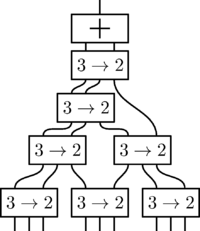
\includegraphics[height=9.1cm]{wallace.png}
  \end{center}

\section{Лекция 6}
\subsection{Нижняя граница на размер функциональной схемы}
\textbf{Линейные программы} - еще один способ задать булеву функцию, в котором удобнее ее рассматривать для всяких оценок. Выберем какой-то базис и переменный, $n$ из которых будут начальными, которые мы будем получать на вход, для остальных заведем правила, по которым они будут вычисляться из предыдущих (расположены эти элементы будут в топологическом порядке).

Пусть у нас есть всего 1 операция в базисе - стрелка Пирса, тогда давайте оценим количество возможных линейных программ для $n$-арной функции с $t$ операциями. Первая операция может быть одной из $n^2$, вторая одной из $(n+1)^2$ и так далее. Тогда сумма: $$n^2*(n+1)^2\dots *(n+t)^2\leq(n+t)^{2t}$$

Подставим в эту формулу константу, например $\frac{2^n}{3n}$: $$\displaystyle\left(n+\frac{2^n}{3n}\right)^{\frac{2*2^n}{3n}}$$

Теперь если мы подсчитаем отношения этого количества ко всем возможным функциям, а их я напомню - $2^{2^n}$, то поймете, что оно довольно быстро стремится к 0.

\subsection{Верхняя граница на размер функциональной схемы}
Пусть у нас есть $n$-арная булева функция для которой мы хотим построить функциональную схему. Заведем две переменные $k$ и $s$ от которых в итоге и будет зависить размер нашей схемы. 

Начнем с того, что представим нашу таблицу истинности, как таблицу c $2^k$ строчками и $2^{n-k}$ столбцами, просто выделив $n-k$ элементов как столбцы. Теперь объединим строчки в блоки по $s$ строк. Хорошо, давайте научимся строить схему для таблицы из одного столбца и $s$ строк. Вариантов, в каком блоке такая подтаблица может оказаться - $\frac{2^k}{s}$, вариантов для каждого блока - $2^s$. Построим демультиплексор, на $k$ элементах, чтобы определять в какой из строк мы оказались, на это уйдет $2^k$ элементов схемы, далее для каждого из типов блоков соберем элементы или, которые в сумме позволят его получить, на это уйдет максимум $s$  умноженное на количество вариаций блоков, то есть: $$\frac{2^k}{s}*2^s*s=2^{k+s}$$

Хорошо, теперь нам нужно собрать столбец целиком, для этого мы возьмем полученные блоки и сделаем с нужными или, всего элеметов или у нас на это уйдет: $$2^{n-k}*\frac{2^k}{s}$$
Осталось собрать столбики в таблицу, чтобы это сделать снова построим демультиплексор, но теперь на $n-k$ вершинах, на что уйдет $2^{n-k}$ элементов, а потом сделаем или для каждого выхода демультиплексора, с нужным для него столбцом, на что уйдет всего $2^{n-k}$ элементов. После этого все результаты надо объединить за еще $2^{n-k}$ элементов.

Получается всего мы потратили: $$2^k+2^{n-k}+2^{k+s}+2^{n-k}*\frac{2^k}{s}+2^{n-k}=O(2^{k+s}+\frac{2^n}{s})$$
Если выбрать $k=\log_2n$, а $k=n-2\log_2n$, то мы и получим сложность порядка $O(\frac{2^n}{n})$.
\section{Лекция 7}
\subsection{Префиксный код}
\textbf{Префиксный код} - принцип однозначного кодирования, при котором для любых двух кодов $a$ и $b$, ни $a$ не является префиксом $b$, ни $b$ не является префиксом $a$.

Доказательство того, что декодирование в таком случае можно сделать однозначно настолько простое, что я оставлю его читателю. 

\subsection{Код Хаффмана}
\textbf{Код Хаффмана} - самый эффективный способ кодировать информацию в том случае, если каждый символ должен кодироваться целым числом бит и, если мы напрямую не пользуемся закономерностями данных, которые кодируем. 

Чтобы закодировать алфавит кодом Хаффмана мы должны иметь частоту появления каждого символа в тексте, который мы кодируем. Построим дерево Хаффмана на основе этих частот, каждый символ станет листом со своим весом, равным частоте появления этого символа в тексте, далее мы будем выполнять следующий алгоритм:
\begin{enumerate}
    \item Находим два элмента без родителя с наименьшим весом
    \item Создаем им родителя с весом, равным суммарному весу этих вершин
\end{enumerate}

Чтобы теперь задать бинарный код для каждого символа напишем на разных ребрах из одной вершины 0 и 1 и теперь, чтобы получить код для какого-то символа, нужно пройтись от корня до этого листа, и конкатенация цифр на ребрах и будет его кодом.
\begin{center}
  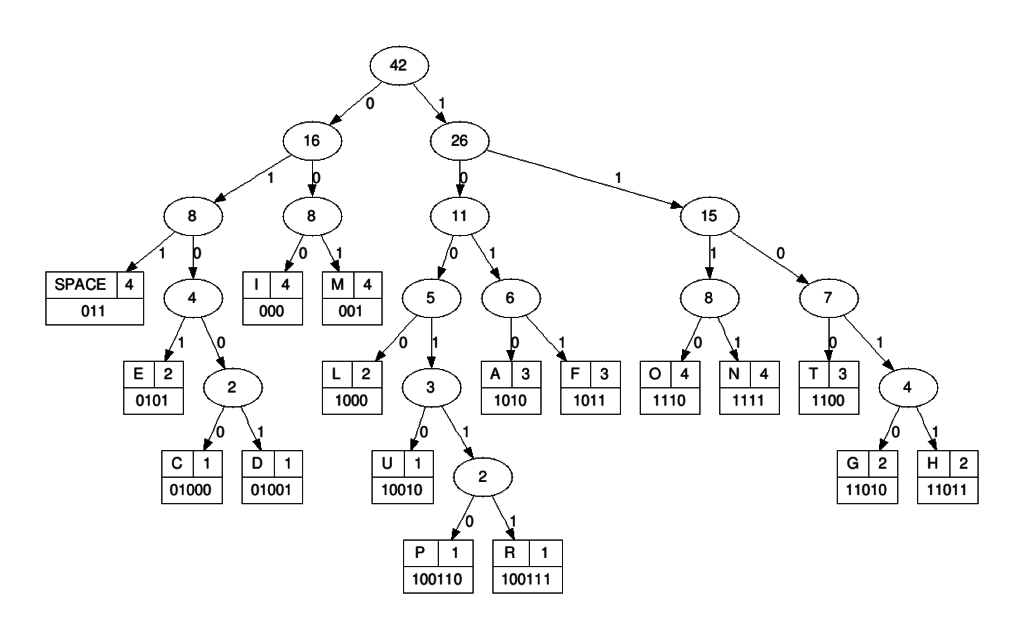
\includegraphics[height=9.1cm]{huffman.png}
\end{center}

Докажем, что это кодирование оптимальнее любого другого. 

\textbf{Лемма} В дереве какого-то из оптимальных кодирований два символа с минимальным весом находятся на максимальной глубине и имеют общего родителя.
\textbf{Доказательство} Пусть это не так, посмотрим на 2 символа на максимальной глубине, имеющие общего родителя (такие обязательно найдутся, так как у нас нет вершин у которых всего 1 потомок, иначе их можно удалить). Эти вершины должны иметь максимальный вес, ведь если это не так, то мы можем поменять их с другими, которые имеют больший вес, а значит предыдущий код был не оптимальным. \textit{QED}

Заметим, что раз 2 вершины с максимальным весом находятся на максимальной глубине, то мы можем заменить их на их родителя, длина кода которого на 1 меньше, а вес тогда будет равен сумме их весов, получается мы уменьшаем общее количество символов на 1. Как раз так и строится дерево Хаффмана, а значит код Хаффмана является оптимальным.
\subsection{Неравенство Крафта-Макмиллана}
В общем случае неравенство Крафта-Макмиллана утверждает: 
Для того, чтобы для набора длин кодовых слов алфавита мощностью $r$: $l_1, l_2 \dots l_n$ существовал однозначно декодируемый код, необходимо и достаточно $$\sum\limits_{i=1}^n2^{-l_i}\leq 1$$
За доказательством \href{https://neerc.ifmo.ru/wiki/index.php?title=%D0%9D%D0%B5%D1%80%D0%B0%D0%B2%D0%B5%D0%BD%D1%81%D1%82%D0%B2%D0%BE_%D0%9C%D0%B0%D0%BA%D0%BC%D0%B8%D0%BB%D0%BB%D0%B0%D0%BD%D0%B0}{сюда}.
\section{Лекция 8}
\subsection{Арифметическое кодирование}
\textbf{Арифметическое кодирование} является улучшенной версией кода Хаффмана, потому что позволяет кодировать символы нецелым числом бит. Алгоритм кодирования устроен так:
\begin{enumerate}
    \item Начните работу с отрезка от 0 до 1.
    \item Поделите отрезок на части в соотношении, равном отношению частот символов
    \item В зависимости от текущего символа в кодируемой строке перейдите к нужному отрезку
    \item Если строка не кончилась перейдите к пункту 2, иначе выберите на полученном отрезке точку вида $\frac{p}{2^q}$ с наименьшим $q$, вашим кодом будет двоичный вектор длины $q$, в котором записано число $p$
\end{enumerate}
\begin{center}
  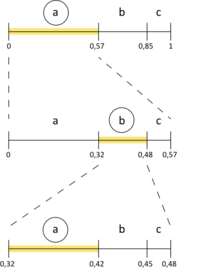
\includegraphics[height=9.1cm]{arif1.png}
\end{center}
Декодирование работает точно так же, мы снова делим отрезок на подотрезки, но теперь мы уже знаем в какой из них нам нужно, так как мы знаем точку, которая ответу принадлежит, перейдем в нужный отрезок и продолжим алгоритм.
\begin{center}
  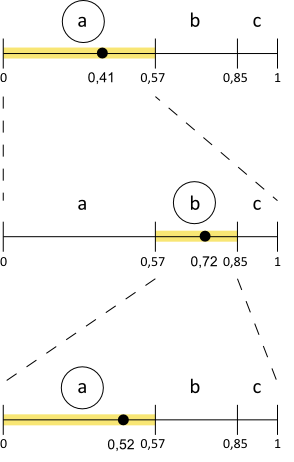
\includegraphics[height=9.1cm]{arif2.png}
\end{center}
\subsection{LZW}
Алгоритм $LZW$ - алгоритм для сжимания данных, основанный на поиске повторяющихся кусков данных и сжимания их. Для сохранения данных о закономерностях предлагается использования буфера. В общем виде алгоритм действия такой:
\begin{enumerate}
    \item Добавление всех символов алфавита в буфер с наименьшими номерами
    \item Инициализируем скользящее окно $X$ как пустую строку
    \item Обработка очередной символа $S$ из текста.
    \item Если $S$ — это символ конца сообщения, то выдать код для $X$, иначе:
    \subitem 4.1. Фраза $XS$ есть в словаре:
    Приписать к $X$ символ $S$, \\Перейти к шагу 3.
    \subitem 4.2 Фразы $XS$ нет в словаре:
    Выдать код для входной фразы $X$, добавить $XY$ в словарь и присвоить $X$ значение $S$. Перейти к Шагу 3. 
\end{enumerate}

Алгоритм декодирования:
\begin{enumerate}
    \item Все возможные символы заносятся в словарь. В скользящее окно $X$
    заносится первый код декодируемого сообщения.
    \item  Считать очередной код $S$ из сообщения.
    \item Если $S$ — это конец сообщения, то выдать символ, соответствующий коду $X$, иначе:
    \subitem 3.1 Если фразы под кодом $XS$ нет в словаре, вывести фразу, соответствующую коду $X$, а фразу с кодом $XS$
    занести в словарь.
    \subitem 3.2 Иначе присвоить входной фразе код $XS$ и перейти к Шагу 2 .
\end{enumerate}
\subsection{Алгоритм Барроуза-Уиллера}
Алгоритм Барроуза-Уиллера также как и $LZW$ производит поиск паттернов в данных, но вместо того, чтобы сжимать их, он просто превращает их в последовательности из одинаковых символов для увеличения эффективности дальнейшего сжатия. Работает он так:
\begin{enumerate}
    \item Выписываем все циклические сдвиги данных в отсортированном порядке.
    \item В качестве результата берем последний столбец, для декодирования запоминаем, какой из символов этого столбца является символом исходной строки.
\end{enumerate} 
\begin{center}
  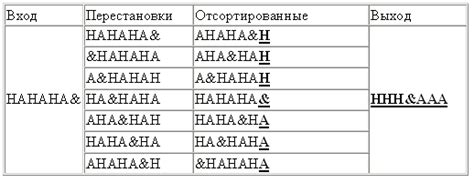
\includegraphics[height=4cm]{barr.jpg}
\end{center}
\textbf{Почему так происходит:} Предположим у нас есть паттерн $s$, который встречается много раз в исходной строке. Тогда если мы возьмем и отрежем у этого паттерна первый символ, пусть он будет $a$, тогда в тех случаях, когда этот символ будет в конце циклического сдвига, остальная часть паттерна будет в его начале, а значит, с большой вероятностью, эти символы будут идти подряд.

Декодирование будет устроено так:
\begin{enumerate}
    \item Изначально у нас будет записан только результат кодирования, который мы отсортируем
    \item Приписываем к полученной таблице слева результат кодирования и сортируем
    \item Если таблица не готова, то перейти к шагу 2, иначе мы берем строку.
\end{enumerate}
Это декодирование основано на том, что у нас выписаны все циклические сдвиги, а значит на самом деле переход от $i$ого столбца к $i+1$ому это какая-то перестановка, причем перестановка постоянная. Тогда эту перестановку можно получить если перебросить первый столбец в конец, у нас получится пара - отсортированный столбец и наш результат левее, значит если так повторять, то мы просто будем применять эту перестановку и получать предыдущий столбец. Сложность декодирования выходит $O(n^2\log n)$.

Но если мы 1 раз построим перестановку и будем применять ее только к элементу последнего столбца, который принадлежит искомой строке, то мы можем восстановить закодированные данные без восстановления всей таблицы, что будет работать уже за $n\log n$.
\section{Лекция 9}
\subsection{Избыточное кодирование}
\textbf{Избыточное кодирование} - кодирования с использованием большего количества информации, чем находится в самом сообщении, для того чтобы уметь находить или исправлять ошибки в данных. 

\textbf{Функция Хэмминга} - функция $H(x,y)$, равная количеству $i$, при которых $x[i]\neq y[i]$. Функция Хэмминга является метрикой для множества строк, так как удовлетворяет всем аксиомам метрики(это просто доказать, так что докажите сами). 

\textbf{Код $c$ обнаруживает $k$ ошибок}, если $k < \min\limits_{\forall x,y \in \mathbb{S}, x\neq y} H\biggl(c(x),c(y)\biggr)$, здесь и далее $\mathbb{S}$ - это множество строк, которые мы кодируем. Докажем, что этот код обнаруживает $k$ ошибок. Возьмем код какой-либо строки - $x$, в которой сделаем $k$ ошибок. Тогда полученная строка $y$ не может быть никаким кодом для любой другой строки, ведь если это так, то у нас есть два кода $x$ и $y$, между которыми расстояние $k$, а значит $k \nless \min\limits_{\forall x,y \in \mathbb{S}, x\neq y} H\biggl(c(x),c(y)\biggr)$.

\textbf{Код $c$ исправляет $k$ ошибок}, если $2k < \min\limits_{\forall x,y \in \mathbb{S}, x\neq y} H\biggl(c(x),c(y)\biggr)$. Работать исправление будет так, мы считаем функцию Хэмминга для всех возможных строк, которые мы могли закодировать, и выбираем ту, до которой расстояние не превышает $k$. Очевидно, что раз мы допускаем, что ошибок в сообщении не больше $k$, то такая строка есть. Докажем что она единственна. Пусть это не так, тогда существует $\exists z\exists x,y\in\mathbb{S}: H(c(x), z) \leq k$ и $H(c(y), z) \leq k$. Тогда из того, что функция Хэмминга у нас метрика, следует: $2k \nless \min\limits_{\forall x,y \in \mathbb{S}, x\neq y} H\biggl(c(x),c(y)\biggr)$.

Для дальнейшего удобства позаимствуем из математического анализа определение шара $B(O, R)$, который будет определен над множеством строк и для которого метрикой будет функция Хэмминга. Объем шара будем обозначать $V(n, R)$, он не зависит от центра, так как $\forall B(O_1,R), B(O_2, R) : \forall x\in B(O_1, R)$ можно привести в соответствие $x \oplus O_1 \oplus O_2$, который принадлежит $B(O_2, R)$, а значит существует биекция между любыми двумя шарами одинакового радиуса, а значит и их объемы равны. 

\underline{\textbf{Лемма.}} Если у нас есть кодирование $c$, обнаруживающее $k$ ошибок, то $\forall x,y \in \mathbb{S}: B(c(x), k) \mathclap{} B(c(y),k) = \varnothing$. Это переосмысление нашего доказательства того, что кодирование, обнаруживающее $k$ ошибок действительно это делает, и определения шара.

\subsection{Теорема: Граница Хэмминга}. Если $c$  - код для множества мощностью $M$, исправляющий $k$ ошибок и использующий $l$ бит для кодирования, то $$M*V(l, k)\leq 2^l$$. 

\textbf{Доказательство.} Просто возьмем шары для каждого закодированного элемента, они все попарно непересекаются. Тогда в них лежит $M*V(l, k)$, что должно быть меньше, чем количество всевозможных кодов, что равно $2^l$

\subsection{Теорема: Граница Гилберта} Если $M*V(l, 2k)\leq 2^l$, то существует код, кодирующий множество мощностью $M$, исправляющий $k$ ошибок и использующий $l$ бит для кодирования.  

\textbf{Доказательство.} Построим такое кодирование. Возьмем любой элемент из множества, которые мы хотим кодировать и выберем для него любой код. Тогда у нас недоступными для выбора следующего кода становится не более $V(lm 2k)$ кодов, выкинем их. Продолжим, пока не зададим каждому элементу свой код. Кодов хватит, так как на выборе $i$ кода мы выбросим не более $(i - 1)*V(l, 2k)$ вершин, и $(i - 1)*V(l, 2k) < M*V(l, 2k)\leq 2^n$. Значит такой код есть.

Общая формула $V(n, R)$: $$V(n, R) = \sum\limits_{i=0}^{R} C_n^i$$

\textbf{Код Хэмминга}. 

\textit{Принцип работы}: Найдем наименьшее $k$, что $k + n < 2^k$. Тогда код Хэмминга кодирует последовательность так: по строке длины $n$ он выдает код длина которого в двоичной системе счисления равна $n + k$, в котором все биты с индексом равным степени двух - контрольные, а остальные n - исходные данные, которые мы бехз изменений перенесем из той строки, которую кодируем. Контрольные биты будем насчитывать так, на $2^i$ позиции будет находиться xor всех чисел, у которых $i$ бит равен 1. Работает все это дело за $O(n\log(n))$.

\begin{center}
  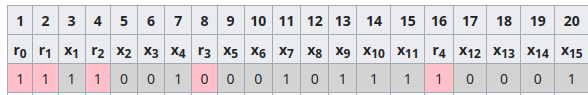
\includegraphics[height=2.1cm]{Hemming_code.png}
\end{center}

\textit{Алгоритм исправления ошибки}: Давайте по полученной строке снова насчитаем контрольные биты по тем же правилам. Теперь давайте найдем индекс изменненого бита. Изначально предположим его равным нулю, начнем проходиться по контрольным битам, если $i$ый насчитанный нами бит не совпадает с тем, что передали нам в строке, то ошибка у нас в числе, у которого в битовой записи на $i$ом месте стоит 1, значит к ответу надо добавить $2^i$. Полученный бит мы просто меняем на противоположный и радуемся. Декодировка также работает за $O(n\log(n))$.

Удивительно, но код Хемминга совпадает с границей Хэмминга, что делает его оптимальным кодированием с исправлением 1 ошибки.

\section{Лекция 10}
\subsection{Комбинаторные объекты}
\textbf{Комбинаторные объекты} - объекты, обладающие между собой некоторыми зависимостями.

Мы будем рассматривать \textbf{линейное представление} комбинаторных объектов - их запись в виде строки над некоторым алфавитом(не обязательно конечным).

Мы хотим научиться:
\begin{enumerate}
\item[1.] Считать количество комбинаторных объектов
\item[2.] Уметь перечислять комбинаторные объекты
\item[3.] Нумеровать комбинаторные объекты 
\item[4.] Выдавать по номеру объект, а по объекту номер
\end{enumerate}
\textbf{Лексикографический порядок} - для двух различных строк $A$ и $B$, строка $A$ лексиграфически меньше строки $B$, если:
\begin{enumerate}
    \item[1.] Строка $A$ - префикс строки $B$
    \item[2.] $\exists i < \min(|A|, |B|): \forall j < i : A_j = B_j$ и $A_i \neq B_i$ 
\end{enumerate}
Очевидно, что этих двух условий достаточно, чтобы задать порядок на строчках. Тогда мы можем задать порядок на всех линейных комбинаторных объектах.

\subsection{Вектора фиксированной длины}
\textbf{Вектор фиксированной длины} - это упорядоченный набор из $n$ (возможно повторяющихся) элементов из алфавита $A$. 

Подсчет количества векторов длины $n$ ни для кого не сотавит затруднения - всего их $|A|^n$.

С нумерацией также проблем не возникает. Пусть $k = |A|$. Тогда давайте зададим каждому элементу из множества $A$ свое число от 0 до $k$. Теперь дадим каждому элементу вектора свой коэффицент, который будет равен $k$ в стенени индекса этого элемента в векторе, то есть для первого элемента это будет $k^0$(для удобства все в 0-индексации), для второго $k^1$ и так далее. Теперь перемножим коэффиценты элементов в векторе на числа, обозначающие данный элемент и получим искомое значение. По факту это запись числа в $k$-ичной системе счисления, и доказательство единственности зашифровки и расшифровки аналогичное.

Из способа нумеровать объекты становится очевиден способы выдавать по номеру объект, мы просто смотрим на остаток от номера по модулю $k$ - это и будет первый элемент вектора, теперь поделим номер на $k$ (с округлением вниз) и аналогично получим второй элемент вектора. Так и продолжим наш алгоритм, пока не получим все элементы вектора.

Если у вас уже упорядочены объекты, то вы можете сортировать их лексикографически.

\subsection{Двоичные вектора без двух единиц подряд}
Не стану вдаваться в подробности, потому что это не очень интересный пример, мы его посмотрим и забудем.

Воспользуемся идеей разделяй и влавствуй и отделим последний элемент нашего вектора. Если это 0, то ограничений на оставшийся вектор нет, а если это 1, то мы точно знаем, что предыдущий элемент нашего вектора это 0, а оставшийся на оставшийся вектор не накладывается никаких ограничений. Тогда мы можем вывести реккурентную формулу: $$F(x) = F(x-1)+F(x-2)$$

Пристальным взглядом можно заметить, что это числа Фиббоначи, а значит мы можем посчитать их по формуле, которую спокойно можно загуглить(не беспокойтесь, на экзамене по дм она вам явно не пригодится).

\subsection{Перестановки}
\textbf{Перестановка} - последовательность длины $n$, такая что все числа в ней от 1 до $n$, при этом в нем нет одинаковых, то есть все числа присутствуют. Можно также это делать не с числами, но полученные перестановки будут изоморфны обычным, так что для удобства дальше мы будем работать только с числами.

Количество перестановок длины $n$ равно $n * (n-1)*(n-2)*\dots *2*1 = n!$.

Очевидно, что перестановки можно лексиграфически нумеровать, так и будем делать.

Давайте научимся по номеру перестановки находить ее. Что происходит, если мы удаляем первый элемент перестановки, у нас остается $(n-1)$ элемент в любом порядке, то есть перестановка на $(n-1)$ элемент. Заведем обозначение на кол-во перестановок длины $k$ - $P_k$. Тогда на первой позиции стоит 1, если итоговый номер не превышает $P_{n-1}$. Если же это не так, давайте выкинем все перестановки, начинающиеся с 1, тогда номер искомой уменьшается на $P_{n-1}$. Для перестановок, начинающихся с 2 мы можем сделать аналогичные умозаключения и понять, стоит в начале перестановки 2 или нет. Продолжая такой алгоритм мы поймем, что стоит на первом месте, тогда можно отбросить это число и продолжить алгоритм для второго числа. Получается такой алгоритм:
\begin{enumerate}
    \item [1.] Имея перестановку длины $n$ и номер искомой перестановки $k$ и набор еще не поставленных чисел $a$ в отсортированном порядке, ставим на первой место перестановки $a[k / P_{n - 1}]$.
    \item[2.] Уменьшаем $n$ на 1, $k$ меняем на $k mod P_{n - 1}$, а из массива $a$ выбрасываем поставленное число и, если он у нас еще не пуст - повторяем алгоритм с начала.
\end{enumerate} 

Ну, раз мы умеем по номеру находить перестановку нам не составит труда запустить обраный алгоритм и узнавать номер перестановки по самой перестановке.

\subsection{Размещения}
\textbf{Размещения} - количество способов упорядоченно выбрать $k$ различных чисел из множества мощностью $n$.

Обозначается $A_n^k$ и имеет формулу $A_n^k = \frac{n!}{(n-k)!}$.

\subsection{Сочетания}
\textbf{Сочетания(биномиальный коэффицент)} - количество способов неупорядоченно выбрать $k$ различных чисел из множества мощностью $n$.

Обозначается $C_n^k$ или $\big(_k^n\big)$ и имеет формулу $C_n^k = \frac{n!}{k!(n-k)!}$(доказательство будет чуть ниже).

Возникают проблемы с тем, что сочетания - не линейный объект и для того, чтобы их решить, введем \textbf{канонизацию}.

\textbf{Канонизация} - довольная абстрактный метод, который говорит: если у нас один и тот же объект может представляться несколькими способами, один из них назовем каноническим, и чтобы упорядочить два объекта, упорядочим их канонические виды. В данном случае, как и во большинстве других, каноническим видом сочетания будет перестановка множества, лексиграфически минимальная, среди всех остальных(Станкевич назвал этот порядок возрастающим, но я буду переиспользовать лексиграфический порядок).

Формула как раз доказывается таким образом, мы берем размещения и говорим, при канонизации у нас все перестановки длины $k$ сводятся к одной строке, значит кол-во сочетаний из n по k = (кол-во размещений из n по k)/(кол-во перестанок длины $k$).

Быстро расскажу про школьный способ считать количество сочетаний, мы снова применяем разделяй и влавствуй для какого-то элемента и если он лежит в множестве, то у нас $C_{n-1}^{k-1}$ способов выбрать оставшиеся элементы, а если он не лежит, то $C_{n - 1}^k$ способов. Снова получаем реккуренту: $$C_n^k=C_{n-1}^k+C_{n-1}^{k-1}$$ для которой можно по индукции доказать, что формула верна, но это выглядит непоследовательно и случайно, а делается довольно просто, поэтому это задания я оставлю читателю, как простейшее упражнение на закрепление формулы сочетаний.

\subsection{Код Грея}
\textbf{Код Грея(для двочиных векторов длины $n$)} - перечисления двочиных векторов в таком порядке, что расстояние Хэмминга между двумя соседними векторами равно 1.

Код Грея называют \textbf{циклическим}, если длина Хэмминга между первой и последней строкой также равна 1.

\textbf{Алгоритм построения циклического кода Грея(зеркального) для двоичных векторов} - Пусть мы хотим построить код Грея для двоичных векторов длины $n$. Построим его для двоичных векторов длины $n-1$ и допишем к ним ко всем в начало 0. Теперь снова этот же код Грея для двоичных векторов длины $n-1$, перевернем его(очевидно, что при этом он останется кодом Грея) и допишем ко всем векторам в нем 1 в начало. Теперь я утверждаю, что я если мы объединим два этих набора векторов, то получим код Грея для векторов длины $n$. Понятно, что коды Грея длины $n-1$, к которым мы приписали один и тот же символ, сломаться не могли, значит, если поломка и произошла, то она произошла на одном из стыков, но это тоже невозможно, ведь там различие только в приписанном в начало символе. Для базы $n=1$ любой порядок векторов будет кодом Грея, значит этот алгоритм может построить код Грея для любого $n$.

\subsection{Формула включений-исключений}
Формально, формула включений-исключений говорит: Если мы умеем считать мощность множеств и мощность их пересечений, то мы можем также посчитать мощность их объединений.

\textbf{Формула}: Для семейства множеств $A_1, A_2, \dots, A_n$: $$\left|\bigcup\limits_{i=1}^{n}A_i\right|=\sum\limits_{I\subset \{1, 2,\dots,n\} I \neq \emptyset}(-1)^{|I|+1}\left(\bigcap\limits_{i\in I}A_i\right)$$
\uline{Доказательство}:
\begin{enumerate}
    \item[] $\displaystyle\left|\bigcup\limits_{i=1}^{n}A_i\right|=\left|\bigcup\limits_{i=1}^{n - 1}A_i \cup A_n\right| = \left|\bigcup\limits_{i=1}^{n - 1}A_i\right| + \left|A_n\right| - \left|\bigcup\limits_{i=1}^{n - 1}(A_i\cap A_n)\right|=\\=\sum\limits_{I\subset \{1, 2,\dots,n-1\}}(-1)^{|I|+1}\left(\bigcap\limits_{i\in I}A_i\right)+|A_n|+\sum\limits_{J\subset \{1, 2,\dots,n\}}(-1)^{|J|+2}\left(\bigcap\limits_{i\in J}A_i\cup A_n\right)$
    
    Посмотрим на эту формулу. Первая сумма это сумма по всем множествам, в которых нет $A_n$, вторая - $A_n$, а третья, это в точности все множества, которые содержат $A_n$ и ещё хоть что-то, причем все с выражения с правильным знаком. Тогда это в точности формула, которую мы хотим доказать.
\end{enumerate}
\section{Лекция 11}
\subsection{Генерация комбинаторных объектов}
Алгоритм един:
\begin{enumerate}
    \item[1.] Проверим является ли полученный префикс комбинаторным объектом.
    \item[2.] Попытаемся дополнить полученный префикс единичным элементом.
    \item[3.] Проверим, является ли полученный префикс корректным префиксом и, если это так, то рекурсивно запустим от него этот алгоритм с первого пункта. 
\end{enumerate}
Код всех генераций ко на языке c++ будет тут после того, как автор конспектов их напишет в лабу и она закончится.
\subsection{Числа Каталана}
Очень классная последовательность, которая очень часто встречается в комбинаторных задачах при подсчете объектов. Формул \textit{iого} числа Каталана много - $\displaystyle C_n = \frac{C^i_{2i}}{i+1}$.

Через подсчет псп - $\displaystyle C_n = \sum\limits_{k=0}^{n-1}C_k*C_{n-1-k}$.

\subsection{Поиск \textit{kого} комбинаторного объекта}
Алгоритм снова един:
\begin{enumerate}
    \item[1.] Проверим является ли полученный префикс комбинаторным объектом, если так, то если номер объекта, который мы ищем - 0, то выведем его и выйдем, иначе просто уменьшим номер объекта, который мы ищем на 1.
    \item[2.] Попытаемся дополнить полученный префикс единичным элементом, которые мы будем обходить в лексикографическом порядке.
    \item[3.] Проверим, является ли полученный префикс корректным префиксом и, если это так, то рекурсивно запустим от него этот алгоритм с первого пункта. 
\end{enumerate}
Этот алгоритм можно немного ускорить, так как нам не обязательно проходить по всем эелементам, если мы умеем быстро считать кол-во ко с каким-то префиксом, то второй пункт можно ускорить.
Код всех поисков ко по их номеру на языке c++ будет тут после того, как автор конспектов их напишет в лабу и она закончится.
\subsection{Получение следующего и предыдущего комбинаторного объекта}
Алгоритм опять един:
\begin{enumerate}
    \item[1.] Найти самый последний элемент, который можно увеличить.
    \item[2.] Увеличить его минимально возможным образом.
    \item[3.] Приписать лексиграфически наименьший хвост.
    
\end{enumerate}

\section{Лекция 12}
\subsection{Разбиение}
\subsubsection{Разбиение на множества}
Разбиение любого множества на набор множеств, так, что каждый элемент исходного множества оказывается ровно в одном множестве набора. 

\subsubsection{Разбиение на слагаемые}
Разбиение числа на множество чисел, так, что сумма этих чисел равна самому числу.

\textit{nое} \textbf{числа Белла} $B_n$ - количество способов разбить на множества множество из n эелементов. 

\textbf{Число Стирлинга 2ого рода} из n по k - $\{_k^n\}=S_2(n, k)$

Формула числа Стирлинга 2ого рода: $$\{_k^n\} = \{_{k - 1}^{n - 1}\}+k*\{_k^{n-1}\}$$
Чтобы это доказать посмотрим на какой-то элемент из $n$, если его удалить и он был один в множестве, то кол-во множеств и элементов уменьшилось и это $\{_{k - 1}^{n - 1}\}$, если же он лежит с кем-то в множестве, то при его удалении мы получим одну и ту же конфигурацию $k$ раз, значит их можно посчитать как $k*\{_k^{n-1}\}$.

Число Белла тогда можно посчитать как: $$B_n = \sum\limits_{k=0}^n\{_k^n\}$$

Число Стирлинга 1ого рода $S_1(n, k)$ - число способов разбить множество мощностью $n$ на $k$ циклов, где цикл - размещения в котором два элемента считаются одинаковыми, если являются циклическими сдвигами друг друга. 

Формула числа Стирлинга 1ого рода: $$\left[_k^n\right] = \left[_{k-1}^{n-1}\right] + (n-1)*[^{n-1}_k]$$
Доказательство этого аналогично доказательству формулы для числа Стирлинга 2ого рода.

Пока что не ясно зачем это, но было обращено внимание на последовательности 1 7 6 1 для чисел Стирлинга 2ого рода, и 6 11 6 1 для чисел Стирлинга 1ого рода, если вы их видите, то с большой вероятностью вы видите числа Стирлинга.

Свойства чисел Стирлинга 1ого рода - $\sum\limits_{k=0}^n[_k^n] = n!$ 
\subsection{Пути Дика}
Рассмотрим плоскость и путь в нем берущий начало в точке (0,0), выполняющий следующие требования:
\begin{enumerate}
    \item [1.] Каждое звено которого направлено вправо на 1 и либо на 1 вверх, либо на 1 вниз.
    \item [2.] Путь Дика обязательно заканчивается в точке с Y-координатой равной нулю.
    \item [3.] Y-координата любой вершины в пути Дика никогда не становится отрицательной.
\end{enumerate}

Проще всего провести аналогию с графиком акций криптовалюты, они обе начинаются с нуля, растут или падают, но в конце концов всегда обесцениваются и оказываются в 0, но при этом не могут быть отрицательны ни в какое время.  

\subsection{Пентагональная формула Эйлера.}

Не будем вдаваться тут особо в подробности о том, что это такое, я скажу так, вас об этом вряд ли спросят, а уж запоминать вы это точно не захотите(Станок мельком что-то об этом упомянул и это скорее та самая легендарная \href{https://dev.mccme.ru/~merzon/mirror/mathtabletalks/files/pentagonal%20(1).pdf}{дополнительная литература по дм}).

\subsection{Бинарные деревья.}
\textbf{Бинарные деревья} - корневые деревья, ограниченные тем, что у каждой вершины не больше двух сыновей, один из которых считается правым, а второй левым. Жесткого ограничения на степень вершины нет, причем четкого предписания, что если сын один, то он обязательно левый или правый тоже нет, поэтому, например, одинаковые по строению деревья, после предписания какие сыновья левые, а какие правые, могут получится разными.

\textbf{Утверждение:} Количество бинарных деревьев на n вершинах -  $C_n$($n$-oe число Каталана)

\textbf{Доказательство:}
\begin{enumerate}
    \item Проведем аналогию с псп, для которого уже все доказано. Пусть вершина - пара открывающейся и закрывающейся скобки, ее левый сын, это та псп, что находится внутри этой пары скобок, а правый сын, та псп, что находится правее нее. Получаем, что из любого дерева мы можем однозначно получить какое-то псп, а также из любой псп можем однозначным образом получить бинарное дерево(если неясно почему, докажите сами), значит это биекция, а значит утверждаемое верно. 
\end{enumerate}

\section{Лекция 13}
\subsection{Перестановки(глубже)}
\subsubsection{Композиция перестановок}
Перестановки можно переменожать, как это было названо на лекции, но здесь далее я буду использовать композицию, потому что это подходит по смыслу больше. При композиции перестановок $a$ и $b$ мы просто переставляем массив по перестановке $a$, а потом по перестановке $b$. Записывается это в обратном порядке - $ba$, а также всегда равно какой-то перестановке $c$, для которой верно: $c[i] = b[a[i]]$, так проще всего и запомнить правильный порядок записи $ba$.

Перестановки \textbf{ассоциативны}, доказывается это так, посмотрим куда попадет $i$ый элемент перестановки: $a(bc)[i]=a[b[c[i]]]$ и $(ab)c[i] = a[b[c[i]]]$.

У перестановок есть \textbf{нулевой элемент}, называемая стабильной перестановкой -  $1, 2, \dots, n$

Также существует и \textbf{обратный элемент}, для перестановок это та перестановка, при композиции с которой наша исходная перестановка $P$ станет стабильной. Доказательство существования такой перестановки может показаться неочевидным, но на самом деле все станет кристально понятно, если мы представим перестановку в виде \href{https://ru.wikipedia.org/wiki/%D0%9E%D1%80%D0%B8%D0%B5%D0%BD%D1%82%D0%B8%D1%80%D0%BE%D0%B2%D0%B0%D0%BD%D0%BD%D1%8B%D0%B9_%D0%B3%D1%80%D0%B0%D1%84}{ориентированного графа}, это представление, кстати, самое удобное, так вот в нем становится понятно, что перестановка это просто набор циклов, и если все ребра в нем повернуть в обратную сторону, то мы также получим какую-то перестановку, которая при композиции с исходной и будет давать стабильную, эту перестановку мы и назовем обратной.

\subsection{Циклические классы}
Мы уже забежали вперед в прошлой секции и представили перестановку в виде графа, так вот \textbf{циклические классы} - это множество циклов данной перестановки, если представить ее в виде графа. Для каждого класса оттуда можно задать его \textbf{мощность} - это просто длина цикла.

\textbf{Инволюция} - перестановка, в которой мощности циклических классов не превышает 2.

\textbf{Порядок перестановки} $P$ - степень $k$, при возведении $P$ в которую у нас получится стабильная перестановка.

Давайте научимся находить порядок перестановки $P$. Представим ее в виде графа и вспомним, что это все циклы какой-то длины. При композиции текущего массива с P мы, по факту, из каждой вершины ходим по ребру, который ведет из этой вершины в перестановке. А так как мы уже помним, что $P$ - это набор циклов каких-то длин, то нам нужно, чтобы итоговое число перемещений по ребрам было кратно всем мощностям циклов, то есть НОК всех мощностей циклов.

\textbf{Важный факт:} Перестановку можно хранить как матрицу, но никто так не делает, так что идем дальше.

\subsection{Теорема Кэли о конечных группах} 
Любая конечная группа $H$ вложена в $S_n$.

\textbf{Уточнение:} $S_n$ - множество всех перестановок из $n$ элементов.

Занумеруем элементы группы $H$, а дальше построим таблицу умножения для этой группы. Теперь сопоставим каждому элементу свою перестановку из $n$ элементов - строку из данной таблицы умножения, соответствующую данному элемент(так как в группе при умножении на разные элементы мы будем получать разные результаты, то это действительно перестановка). Сопоставим элементу $a$ перестановку $L_a$, тогда знаем мы такое: $L_{ab}h=(ab)h=a(bh)=L_aL_bh$, значит $L_{ab}=L_aL_b$.

\section{Лекция 14}
\subsection{Подсчет с точностью до действия группы}
На группе заводятся действия, которые удовлетворяют следующим аксиомам:
\begin{enumerate}
    \item[1)] $h(g(x))=(h*g)(x)$, набор действий это группа и для них определено умножение
    \item[2)] $ex=x$, существует нейтральный элемент
\end{enumerate}
Для действия может быть \textbf{неподвижная точка}, для которой верно:$$I_g=\{x|x : gx=x\}$$
Для элемента $x$ существует \textbf{стабилизатор} - действия, которые его не изменяют:$$St_x = \{g|gx=x\}$$
Мы получили отношения эквивалентности, это можно проверить, проверив рефлексивность транзитивность и симметричность.
$X/G$ - множество классов эквивалентности, называемая \textbf{орбитами}.
\subsection{Лемма Бёрнсайда}
Формула - $$\displaystyle\left|X/G\right|=\frac{\sum\limits_{g\in G}|I_g|}{|G|}$$ Выглядит это буквально как среднее арифметическое размеров групп, им оно на самом деле и является.

Доказательство:

Нарисуем таблицу всех действий на всевозможные объекты. Рассмотрим какой-нибудь столбец элемента $x_i$, это будет его орбита, из-за отношения эквивалентности. Некоторые орбиты могут оказаться одинаковыми - для эквивалентных элементов, если будем находить несколько таких, то выкинем повторяющиеся. Столбцов тогда останется столько, сколько у нас всего орбит - $|X/G|$. Строк - $|G|$. А каждый элемент встречается теперь всего один раз, в том столбце, на которой орбите он лежит, но лежит он там столько раз, сколько действий превращают его в самого себя, то есть $|St_x|$ раз. Тогда мы получили такую формулу: $|X/G|*|G|=\sum\limits_x{St_x}$. Ну а эта формула уже очевидно приводится к нужной, так как сумма мощностей неподвижных точек по всем $g$ равна сумме стабилизаторов по всем $x$.  
\subsection{Теорема Пойя}
Число орбит - $|X/G| = \frac{1}{|G|}\sum\limits_g{S^{C(G)}}$ или $|X/G| = \frac{1}{|G|}\sum\limits_{i=1}^n{k_i*S^{i}}$, где $k_i$ - количество действий, перестановка которых имеет k циклов. 
Тут также доказательство я лучше вынесу в удобную \href{https://neerc.ifmo.ru/wiki/index.php?title=%D0%9B%D0%B5%D0%BC%D0%BC%D0%B0_%D0%91%D1%91%D1%80%D0%BD%D1%81%D0%B0%D0%B9%D0%B4%D0%B0_%D0%B8_%D0%A2%D0%B5%D0%BE%D1%80%D0%B5%D0%BC%D0%B0_%D0%9F%D0%BE%D0%B9%D0%B0}{ссылочку}.
\end{document}  
